\section{Aritmetica}
\subsection{Propiedades de los Números Reales}
\begin{multicols}{2}
  \begin{itemize}[leftmargin=*,noitemsep,topsep=0pt]
    \item \textbf{Conmutatividad}:
      \begin{align*}
        a + b &= b + a \\
        a \cdot b &= b \cdot a
      \end{align*}

    \item \textbf{Asociatividad}:
      \begin{align*}
        (a + b) + c &= a + (b + c) \\
        (a \cdot b) \cdot c &= a \cdot (b \cdot c)
      \end{align*}

    \item \textbf{Distributividad}:
      \begin{align*}
        a \cdot (b + c) &= a \cdot b + a \cdot c \\
        (b + c) \cdot a &= b \cdot a + c \cdot a
      \end{align*}

    \item \textbf{Elementos neutros}:
      \begin{align*}
        a + 0 &= a \\
        a \cdot 1 &= a
      \end{align*}

    \item \textbf{Inversos}:
      \begin{align*}
        a + (-a) &= 0 \\
        a \cdot a^{-1} &= 1 \quad (a \neq 0)
      \end{align*}
  \end{itemize}

  \subsection{Binomio}
  $$\combinat{n}{k}=\dfrac{n!}{(n-k)!n!} \quad n,k \in \mathbb{Z}; n>k$$
  $(x+y)^n=\combinat{n}{0}x^{n-0}y^0+\combinat{n}{1}x^{n-1}y^1+\combinat{n}{n-1}x^{n-(n-1)}y^{(n-1)}$ generalizando podria expresarse como
  $$(x+y)^n=\sum\limits_{k=0}^n \combinat{n}{k} x^{n-k}y^k$$

\subsection{Conjunto}
\[
\begin{array}{l}
  \mathbb{C} \left\{
    \begin{array}{l}
      \mathbb{R} \left\{
        \begin{array}{l}
          \text{Racional } (\mathbb{Q}) \left\{
            \begin{array}{l}
               \mathbb{Z} \left\{
                \begin{array}{l}
                  \text{Natural } (\mathbb{N}) \left\{
                    \begin{array}{l}
                      1\\
                      \text{Primos}\\
                      \text{Compuestos}
                    \end{array}
                  \right. \\[4pt]
                  \text{Enteros -}\\
                  \text{01}
                \end{array}
              \right. \\[4pt]
              \text{Fraccionarios} \left\{
                \begin{array}{l}
                  \text{Propios}\\
                  \text{Impropios}
                \end{array}
              \right.
            \end{array}
          \right. \\[4pt]
          \text{Irracionales}
        \end{array}
      \right. \\[4pt]
      i
    \end{array}
  \right.
\end{array}
\]

              \subsection{Criterios de divisibilidad}
              2. Su ultima cifra es cero o par\\
              3. Suma de sus cifras mult. de 3 \\
              4. Sus ultimas cifras son 00 o mult de 4, si es par y su mitad es par\\
              5. Su ultima cifra es 0 o 5\\
              6. Si es div por 2 y 3\\
              7. La diferencia entre el numero formado por todas las cifras menos la ultima y el doble de la ultima es 0 o 7\\
              9. La suma de sus cifras es 9\\
              11. Si al sumar las cifras colocadsa en el lugar par y restarles la sumas de las cifras en lugar impar es 0 o 11
              \columnbreak
              \subsection*{División Sintética}
              \begin{itemize}[leftmargin=*]

                \item \textbf{Propósito}: Dividir $P(x)$ entre $(x - c)$
                \item \textbf{Pasos}:
                  \begin{enumerate}
                    \item Escribir coeficientes de $P(x)$ (ordenados)
                    \item Bajar el primer coeficiente
                    \item Multiplicar por $c$ y sumar a la siguiente columna
                    \item Repetir hasta terminar
                  \end{enumerate}

                \item \textbf{Ejemplo}:
                  Dividir $2x^3 - 6x^2 + 2x - 1$ entre $(x-3)$ \\
                  $
                  \begin{array}{r|rrrr}
                    3 & 2 & -6 & 2 & -1 \\
                    &   & 6 & 0 & 6 \\
                    \hline
                    & 2 & 0 & 2 & 5 \\
                  \end{array}$ \\
                  Resultado: $2x^2 + 0x + 2$ con residuo $5$
              \end{itemize}

              \subsection*{Teorema del Residuo}
              \begin{itemize}[leftmargin=*]
                \item $P(c) = \text{Residuo de } P(x) \div (x - c)$
              \end{itemize}

              \subsection*{Teorema del Factor}
              \begin{itemize}[leftmargin=*]
                \item $(x - c)$ es factor $\iff P(c) = 0$
              \end{itemize}

              \subsection*{Raíces de Polinomios}
              \begin{itemize}[leftmargin=*]
                \item \textbf{Teorema Fundamental}:
                  Todo polinomio de grado $n$ tiene $n$ raíces en $\mathbb{C}$

                \item \textbf{Raíces Racionales}:
                  Para $P(x) = a_nx^n + \cdots + a_0$, las posibles raíces racionales son $\pm \frac{p}{q}$ donde $p|a_0$ y $q|a_n$

                \item \textbf{Multiplicidad}:
                  Si $(x-c)^k$ es factor pero $(x-c)^{k+1}$ no lo es, $c$ es raíz de multiplicidad $k$
              \end{itemize}
              \subsection{Series}
              \subsubsection{Taylor}

              Para 1D
              $$f(x+ \Delta x)=f(x_0)+\Delta x \left.\dfrac{df(x)}{dx}\right|_{x=x_0}+\dfrac{\Delta x^n}{n!} \left.\dfrac{d^nf(x)}{dx^n}\right|_{x=x_0}$$
              Para 2D (hasta segundo orden)
              $$
              f(x_0+\Delta x, y_0+ \Delta y)=f(x_0,y_0)+\Delta x\left.\dfrac{\partial f}{\partial x}\right|_{(x_0,y_0)}+\Delta y\left.\dfrac{\partial f}{\partial y}\right|_{(x_0,y_0)}
              $$
              $$
              +\dfrac{\Delta x^2}{2!} \left. \dfrac{\partial^2 f}{\partial x^2}\right|_{(x_0,y_0)}+\Delta x\Delta y \left. \dfrac{\partial^2 f}{\partial x\partial y}\right|_{(x_0,y_0)}+\dfrac{\Delta y^2}{2!} \left. \dfrac{\partial^2 f}{\partial y^2}\right|_{(x_0,y_0)}+\cdots
              $$

            \end{multicols}

            \newpage
            \section{Identidades Trigonométricas}
            \begin{multicols}{2}

              \fmSubSec{Identidades de Suma}
              \begin{itemize}[leftmargin=*,noitemsep,topsep=0pt]
                \item \textbf{Seno de la suma}:
                  \[ \sin(a \pm b) = \sin a \cos b \pm \cos a \sin b \]

                \item \textbf{Coseno de la suma}:
                  \[ \cos(a \pm b) = \cos a \cos b \mp \sin a \sin b \]

                \item \textbf{Tangente de la suma}:
                  \[ \tan(a \pm b) = \dfrac{\tan a \pm \tan b}{1 \mp \tan a \tan b} \]
              \end{itemize}

              \fmSubSec{Identidades de Ángulo Doble}
              \begin{itemize}[leftmargin=*,noitemsep,topsep=0pt]
                \item \textbf{Seno}:
                  \[ \sin(2a) = 2 \sin a \cos a \]

                \item \textbf{Coseno}:
                  \[ \cos(2a) = \cos^2 a - \sin^2 a \]
                  \[ = 2\cos^2 a - 1 \]
                  \[ = 1 - 2\sin^2 a \]

                \item \textbf{Tangente}:
                  \[ \tan(2a) = \dfrac{2\tan a}{1 - \tan^2 a} \]
              \end{itemize}


              \fmSubSec{Identidades de Ángulo Mitad}
              \begin{itemize}[leftmargin=*,noitemsep,topsep=0pt]
                \item \textbf{Seno}:
                  \[ \sin\left(\dfrac{a}{2}\right) = \pm \sqrt{\dfrac{1 - \cos a}{2}} \]

                \item \textbf{Coseno}:
                  \[ \cos\left(\dfrac{a}{2}\right) = \pm \sqrt{\dfrac{1 + \cos a}{2}} \]

                \item \textbf{Tangente}:
                  \[ \tan\left(\dfrac{a}{2}\right) = \pm \sqrt{\dfrac{1 - \cos a}{1 + \cos a}} \]
                  \[ = \dfrac{1 - \cos a}{\sin a} \]
                  \[ = \dfrac{\sin a}{1 + \cos a} \]
              \end{itemize}
              \columnbreak

              \fmSubSec{Identidades Fundamentales}
              \begin{itemize}[leftmargin=*,noitemsep,topsep=0pt]
                \item \textbf{Pitagóricas}:
                  \[ \sin^2 a + \cos^2 a = 1 \]
                  \[ 1 + \tan^2 a = \sec^2 a \]
                  \[ 1 + \cot^2 a = \csc^2 a \]
              \end{itemize}
              
              \fmSubSec{Producto a Suma}
              \begin{itemize}[leftmargin=*,noitemsep,topsep=0pt]
                \item \textbf{Seno por Coseno}:
                  \[ \sin a \cos b = \dfrac{1}{2}[\sin(a+b) + \sin(a-b)] \]
                \item \textbf{Coseno por Coseno}:
                  \[ \cos a \cos b = \dfrac{1}{2}[\cos(a+b) + \cos(a-b)] \]
                \item \textbf{Seno por Seno}:
                  \[ \sin a \sin b = \dfrac{1}{2}[\cos(a-b) - \cos(a+b)] \]
              \end{itemize}

                \fmSubSec{Suma a Producto}
              \begin{itemize}[leftmargin=*,noitemsep,topsep=0pt]
                \item \textbf{Suma de senos}:
                  \[ \sin a + \sin b = 2\sin\left(\dfrac{a+b}{2}\right)\cos\left(\dfrac{a-b}{2}\right) \]
                \item \textbf{Suma de cosenos}:
                  \[ \cos a + \cos b = 2\cos\left(\dfrac{a+b}{2}\right)\cos\left(\dfrac{a-b}{2}\right) \]
              \end{itemize}

            \fmSubSec{Triangulo oblicuangulo}
    \begin{multicols}{2}
        
    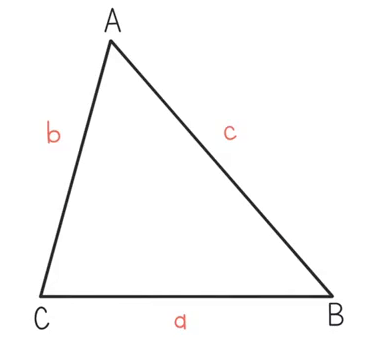
\includegraphics[width=1\linewidth]{src/Obli.png}
\columnbreak
            \begin{itemize}
                \item Ley de Senos
                $$\dfrac{a}{\sin A}=\dfrac{b}{\sin B}=\dfrac{c}{\sin C}$$
                \item Ley de cosenos
                $$
                \begin{aligned}
                a^2 &= b^2 + c^2 - 2bc \cos A \\
                b^2 &= a^2 + c^2 - 2ac \cos B \\
                c^2 &= a^2 + b^2 - 2ab \cos C
                \end{aligned}
                $$
            \end{itemize}
    \end{multicols}

            \end{multicols}
            \newpage
            \section{Complex}
            \begin{multicols}{2}

              \fmSubSec{Definición Básica}
              \begin{itemform}[leftmargin=*]
                \item \textbf{Forma binomial}:
                  $$ z = a + bi \quad (a,b \in \mathbb{R})$$
                \item \textbf{Unidad imaginaria}:
                  $$ i^2 = -1 \rightarrow -i=\dfrac{1}{i}$$
              \end{itemform}

              \fmSubSec{Conjugado Complejo}
              \begin{itemform}[leftmargin=*]
                \item \textbf{Definición}:
                  $$ \overline{z} = a - bi $$
                \item \textbf{Propiedades clave}:
                  \begin{align*}
                    \overline{z_1 \pm z_2} &= \overline{z_1} \pm \overline{z_2} \\
                    \overline{z_1 z_2} &= \overline{z_1} \cdot \overline{z_2} \\
                    \overline{\left(\frac{z_1}{z_2}\right)} &= \frac{\overline{z_1}}{\overline{z_2}} \\
                    z \cdot \overline{z} &= |z|^2 \\
                    \overline{\overline{z}} &= z \\
                    \text{Re}(z) = \frac{z + \overline{z}}{2} &\quad
                    \text{Im}(z) = \frac{z - \overline{z}}{2i}
                  \end{align*}
              \end{itemform}

              \fmSubSec{Representaciones}
              \begin{itemform}[leftmargin=*]
                \item \textbf{Polar}:
                  $$ z = |z|(\cos\theta + i\sin\theta) $$
                \item \textbf{Exponencial}:
                  $$ z = |z|e^{i\theta} $$
                \item \textbf{Fasorial:}
                $$z=|z| \angle \theta$$
              \end{itemform}
    Nótese que $|Z|>0$ por lo que si es negativo se hace $$-Z\angle \theta \Rightarrow Z\angle (\theta + 180^{\circ})$$
              \columnbreak

              \fmSubSec{Operaciones Algebraicas}
              \begin{itemform}[leftmargin=*]
                \item \textbf{Suma/Resta}:
                  $$ (a+bi) \pm (c+di) = (a \pm c) + (b \pm d)i $$

                \item \textbf{Multiplicación}:
                  $$ (a+bi)(c+di) = (ac-bd) + (ad+bc)i $$
                \item \textbf{Multiplicación Conjugada}:
                  $$ (a+bi)(c-di) = (ac+bd) + (bc-ad)i $$

                \item \textbf{División}:
                  $$ \frac{a+bi}{c+di} =\frac{a+bi}{c+di} \dfrac{c-di}{c-di} = \frac{(a+bi)(c-di)}{c^2+d^2} $$
              \end{itemform}

              \fmSubSec{Potencias y Raíces}
              \begin{itemform}[leftmargin=*]
                \item \textbf{Fórmula de De Moivre}:
                  $$ z^n = |z|^n \left[\cos(n\theta) + i\sin(n\theta)\right] $$

                \item \textbf{Raíces n-ésimas}:
                  $$ \sqrt[n]{z} = |z|^{1/n} \left[\cos\left(\frac{\theta + 2k\pi}{n}\right) + i\sin\left(\frac{\theta + 2k\pi}{n}\right)\right] $$
                  para $k = 0,1,\dots,n-1$
                  \[
\omega^k = e^{\frac{2\pi i k}{n}} = \cos\left(\frac{2\pi k}{n}\right) + i\sin\!\left(\frac{2\pi k}{n}\right)
\]

              \end{itemform}

              \fmSubSec{Propiedades del Módulo}
              \begin{itemform}[leftmargin=*]
                \item $|z| = \sqrt{a^2 + b^2}$
                \item $|z_1 z_2| = |z_1||z_2|$
                \item $\left|\frac{z_1}{z_2}\right| = \frac{|z_1|}{|z_2|}$
                \item $|z^n| = |z|^n$
              \end{itemform}

            \end{multicols}
            \newpage

            \begin{multicols}{2}
              \section{Calculo I}
              \subsection{Funciones}

              $
              \begin{aligned}
                f : &\mathbb{R} \rightarrow \mathbb{R} \quad \quad \Gamma_f=\{x,f(x) | x \in Dom_f\}\\
                &x \longmapsto f(x)    \quad \quad  D_f = \{ x \in \mathbb{R} | f(x) \in \mathbb{R} \}\\
              \end{aligned}
              $
              \subsection{Operaciones}
              $(f \pm g) (x) \ | \ (f \cdot g) (x)$
              \\
              $
              \begin{aligned}
                f \pm g \ | \ f \cdot g: &\mathbb{R} \rightarrow \mathbb{R}\\
                &x \longmapsto (f\pm g)(x) = f(x) \pm g(x) \\
                &x \longmapsto (f\cdot g)(x) = f(x) \cdot g(x)
              \end{aligned}
              \\
              Dom_{f \pm g}= Dom_f \cap Dom_g \\  Dom_{f \cdot g}= Dom_f \cap Dom_g
              $
              \\\\
              $\left(\frac{f}{g}\right) (x)$
              \\
              $
              \begin{aligned}
                \frac{f}{g} : &\mathbb{R} \rightarrow \mathbb{R}\\
                &x \longmapsto \left(\frac{f}{g}\right)(x) = \frac{f(x)}{g(x)}
              \end{aligned}
              \\
              Dom_{\frac{f}{g}}= Dom_f \cap Dom_g \backslash \{ x \in Dom_g | g(x) = 0\}
              $
              \\\\
              $(f \circ g) (x)$
              \\
              $
              \begin{aligned}
                f \circ g : &\mathbb{R} \rightarrow \mathbb{R}\\
                &x \longmapsto (f\circ g)(x) = f(g(x))
              \end{aligned}
              \\
              Dom_{f \circ g}= \{ x \in Dom_g | g(x) \in Dom_f\} \subseteq Dom_f
              $

              \subsection{Continuidad}
              \begin{minipage}{0.3\textwidth}\RaggedRight
                Observemos que \\$\lim_{x\to a} f(x)=f(a)$\\
                $
                \begin{aligned}
                  L1&=L2\\
                  \lim_{x\to a^-}f(x) &=\lim_{x\to a^+}f(x)\\
                  L_1 \exists &\wedge L_2 \exists \ \therefore L \exists\\
                \end{aligned}$

                Ademas observamos que el $\lim_{x\to b}f(x) \nexists$\\
              \end{minipage}
              \noindent
              \begin{minipage}{0.2\textwidth}
                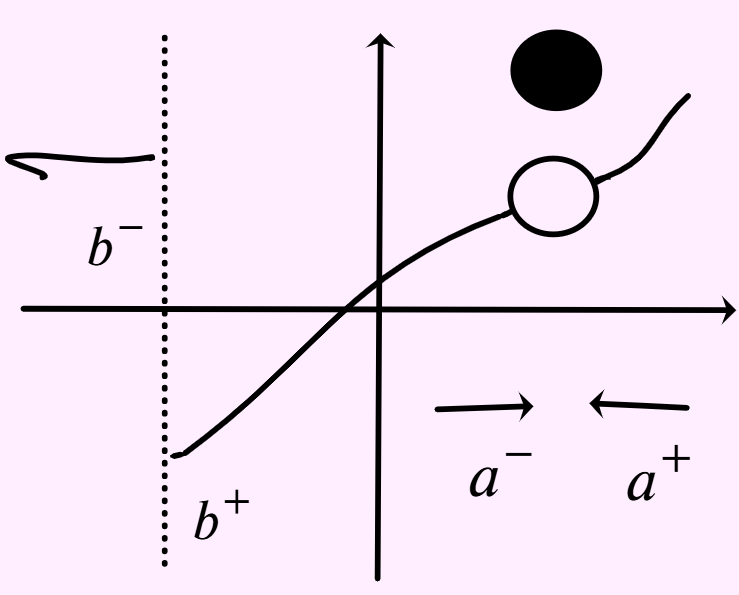
\includegraphics[scale = 0.17]{src/Conti.png}
              \end{minipage}
              \hfill%
              \\\\
              \textbf{Axiomas de Continuidad}
              \begin{itemize}
                \item $f(a) \ \exists \ (a \in Dom_f)$
                \item $\lim_{x \to a} f(x) \ \exists$
                \item $\lim_{x \to a} f(x) = f(a)$
              \end{itemize}
              $
              \begin{aligned}
                \text{Sea f}&: \mathbb{R} \to \mathbb{R} \text{ función}    \\
                &I \subseteq Dom_f \text{ Intervalo}
              \end{aligned}
              $
              \begin{enumerate}
                \item Si I es intervalo abierto entonces f es continua en I si es continua en cada punto I.
                \item Si I es intervalo cerrado entonces f es continua si:
                  \begin{itemize}
                    \item f es continua en (a,b)
                    \item $\lim_{x\to a^+} f(x)=f(a) $\\
                      $\lim_{x\to b^-} f(x) =f(b)$

                  \end{itemize}
              \end{enumerate}
              \columnbreak

              \subsection{Teoremas}
              \begin{itemize}
                \item Constante\\
                  $\lim_{x \to a} k = k \quad \quad a,k \in \mathbb{R}$
                \item Identidad\\
                  $\lim_{x \to a} x = a \quad \quad a \in \mathbb{R}$
                \item Constante por $f(x)$\\
                  $\lim_{x \to a} kf(x) = k\lim_{x \to a} f(x) \quad \quad k \in \mathbb{R}\ \ L(f(x)) \exists$
                \item Suma Resta Producto\\
                  $\lim_{x \to a} [f(x)\pm g(x)] = \lim_{x \to a} f(x) \pm \lim_{x \to a} g(x) $
                \item Cociente de funciones\\
                  $\lim_{x \to a} \dfrac{f(x)}{g(x)} = \dfrac{\lim_{x \to a} f(x)}{\lim_{x \to a} g(x)} \\\lim_{x\to a}(f(x)), \lim_{x\to a}(g(x)) \ \exists \  \wedge\ \lim_{x\to a}(g(x)) \ne 0 $
                \item Funcion Racional\\
                  $\lim_{x \to a} \dfrac{\mathbb{P}(x)}{\mathbb{Q}(x)}=\dfrac{\lim_{x\to a} \mathbb{P}(x)}{\lim_{x\to a} \mathbb{Q}(x)}$
                \item Exponentes\\
                  $\lim_{x\to a}(f(x))^n=(\lim_{x\to a}(f(x)))^n$
                \item Raices de indice par\\
                  $\lim_{x\to a} \sqrt[n]{f(x)}=\sqrt[n]{\lim_{x\to a} f(x)} \\ f(x) \ge 0, n=2k$
                \item Division entre cero \\
                  $\dfrac{f(x)}{g(x)}=
                  \begin{matrix}
                    f(x) & g(x) & case \\
                    0 & 0 &\text{Ind. tipo } 0/0 \\
                    0 & g(x)  & 0\\
                    f(x) & 0 & \nexists\\
                  \end{matrix}$
              \end{itemize}

              \subsection{Limites al Infinito}
              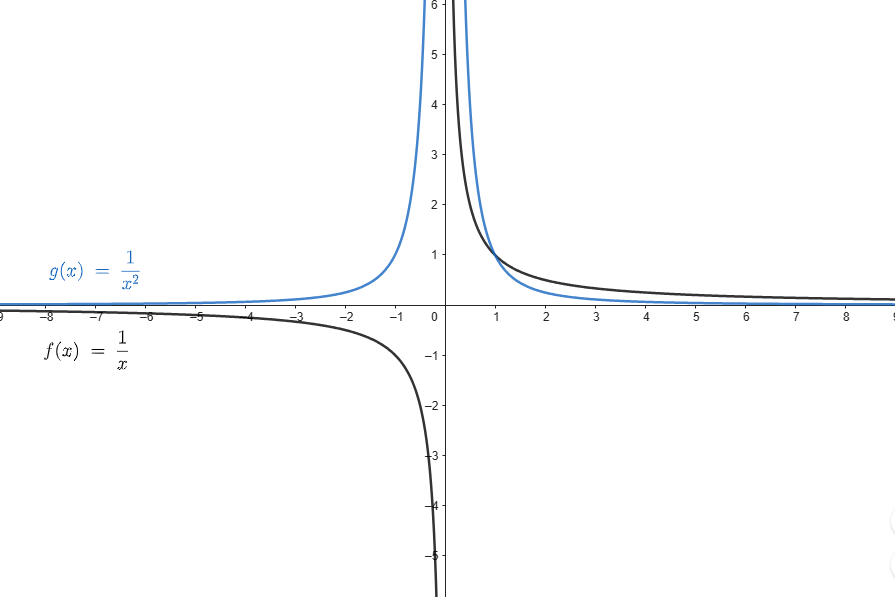
\includegraphics[scale = 0.35]{src/plotfavor.png}\\
              Para $ n\in \mathbb{R}$\\
              $\lim_{x\to \infty} x^n =\lim_{x \to 0^+} \dfrac{1}{x^n}= \lim_{x\to a^+} \dfrac{1}{(x-a)^n} = \infty $\\
              $\lim_{x\to -\infty} x^n =\lim_{x \to 0^-} \dfrac{1}{x^n}= \lim_{x\to a^-} \dfrac{1}{(x-a)^n} =\left\{
                \begin{aligned}
                  &+\infty \text{ si n es par} \\
                  &-\infty \text{ si n es impar}
                \end{aligned} \right. $\\

              \end{multicols}
              \newpage
              \section{Calculus II}
              \begin{vwcol}[widths={0.3,0.6}, sep=.5cm, justify=flush,rule=2pt,indent=0em]
                \begin{align*}
                  &D_x(k) = 0 \\
                  &D_x[kf(x)] = k \cdot D_x[f(x)] \\
                  &D_x[f(g(x))] = f'(g(x)) \cdot D_x[g(x)]
                \end{align*}

                \begin{align*}
                  \\&D_x[g(x)\cdot h(x)] = g(x)\cdot h'(x) + g'(x) \cdot h(x) \\
                  &D_x\left[\frac{h(x)}{g(x)}\right] =  \frac{g(x)\cdot h'(x) - g'(x)\cdot h(x)}{g(x)^2}=\frac{h'(x)}{g(x)}-\frac{g'(x)\cdot h(x)}{g(x)^2}               \\
                  &D_x[f(x) \pm g(x)] = D_x[f(x)] \pm D_x[g(x)]
                \end{align*}
              \end{vwcol}

              \textbf{\\}
              %
              \begin{vwcol}[widths={0.2,1.6,0.6}, sep=.5cm, justify=flush,rule=2pt,indent=0em]
                \begin{align*}
                  &Definition\\
                  &\lim_{{h \to 0}} \frac{f(x+h) - f(x)}{h}\\
                  &D_x[\ln(u)] = \frac{u'}{u} \\
                  &D_x[\log(u)] = \frac{\log(e) \cdot u'}{u} \\
                  &D_x[a^u] = a^u \cdot \ln(a) \cdot u' \\
                  &D_x[e^u]=e^v\cdot v'
                \end{align*}
                \begin{align*}
                  \\&D_x[\sin(u)] = u'\cdot \cos(u)
                  \\&D_x[\cos(u)] = -u'\cdot \sin(u)
                  \\&D_x[\tan(u)] = u'\cdot \sec^2(u)_{[1]}
                  \\&D_x[\arcsin(u)] = \frac{u'}{\sqrt{1-u^2}}
                  \\&D_x[\arccos(u)] = \frac{-u'}{\sqrt{1-u^2}}
                  \\&D_x[\arctan(u)] = \frac{u'}{1+u^2}
                \end{align*}
                \begin{align*}
                  \\&D_x[\csc(u)] = -u'\cdot \csc(u) \cdot \cot(u)
                  \\&D_x[\sec(u)] = u'\cdot \sec(u) \cdot \tan(u)
                  \\&D_x[\cot(u)] = -u'\cdot \csc^2(u)
                  \\&D_x[\arccsc(u)] = \frac{-u'}{u\cdot \sqrt{(u^2-1)}}
                  \\&D_x[\arcsec(u)] = \frac{u'}{u\cdot \sqrt{u^2-1}}
                  \\&D_x[\arccot(u)] = \frac{-u'}{1+u^2}
                \end{align*}
              \end{vwcol}

              \[\sec^2(u)=\sec(u)^2 \ne \sec(u^2)\]
              Every result is +C
              \begin{vwcol}[widths={0.2,0.6,0.6,0.2}, sep=.5cm, justify=flush,rule=2pt,indent=0em]
                \begin{align*}
                  &Definition\\
                  &\int_a^b f(x) dx = \lim_{{n \to \infty}} \sum_{{i=1}}^{n} f(x_{i-1}) \Delta x\\
                  &=F(b)-F(a)\\
                  &\int kdx = k\int  dx = kx\\
                  &\int (u + v)dx = \int u dx + \int vdx \\
                  &\int x^ndx=\frac{x^{n+1}}{n+1} \textbf{ } \int \frac{dv}{v}dx= \ln(v)\\
                  &\int a^vdx=\frac{a^v}{\ln(a)} \textbf{ } \int e^vdx=e^v
                \end{align*}
                \begin{align*}
                  \\&\int \sin(u)du = -\cos(u)
                  \\&\int \cos(u)du = \sin(u)
                  \\&\int \tan(u)du = \ln(\sec(u))
                  \\&\int \frac{du}{\sqrt{1-u^2}} = \arcsin(u)
                  \\&\int -\frac{du}{\sqrt{1-u^2}} = \arccos(u)
                  \\&\int \frac{du}{1+u^2} = \arctan(u)
                \end{align*}
                \begin{align*}
                  \\&\int \csc(u)du = -\cot(u)
                  \\&\int \sec(u)du = \tan(u)
                  \\&\int \cot(u)du = \ln(\sin(u))
                \end{align*}
                \begin{align*}
                  \\&\int \csc(u)\cdot \cot(u) du = -\csc(u)
                  \\&\int \sec(u)\cdot \tan(u) = \tan(u)
                  \\&\int \cot(u)du = \ln(\sin(u))
                  \\&\int -\frac{du}{u\cdot \sqrt{(u^2-1)}} = \arccsc(u)
                  \\&\int \frac{du}{u\cdot \sqrt{u^2-1}} = \arcsec(u)
                  \\&\int -\frac{du}{1+u^2} = \arccot(u)
                \end{align*}
              \end{vwcol}
              \textbf{\\}
              \begin{table}[h]
                \begin{align*}
                  \textbf{Integration by parts}\\
                  \int udv = uv- \int vdu
                \end{align*}

                \begin{tabular}{c|c|c}
                  u& Inv. Trig&$\arcsin,\arctan$\\
                  &  Logarithmic & $\ln,\log$\\
                  &  Algebraic & $x^2,x^{-3}$\\
                  &  Trigonometric& $\sin,\cos$ \\
                  dv& Exponential& $e^{2x},3^{2x}$\\
                \end{tabular}
              \end{table}

              \newpage
              \section{Álgebra Matricial}
              \begin{multicols}{2}

                \fmSubSec{Definiciones Básicas}
                \begin{itemform}[leftmargin=*]
                \item \textbf{Matriz } $m \times n$:
                  $$ A = [a_{ij}]_{m \times n} $$

                \item \textbf{Matriz identidad}:
                  $$ I_n = (\delta_{ij}) \quad \delta_{ij} =
                  \begin{cases}
                    1 & i=j \\
                    0 & i \neq j
                  \end{cases} $$

                \item \textbf{Traza}:
                  $$ \text{tr}(A) = \sum_{i=1}^n a_{ii} $$
                \end{itemform}

                \fmSubSec{Operaciones Fundamentales}
                \begin{itemform}[leftmargin=*]
                \item \textbf{Suma}:
                  $$ (A+B)_{ij} = a_{ij} + b_{ij} $$

                \item \textbf{Producto por escalar}:
                  $$ (\lambda A)_{ij} = \lambda a_{ij} $$

                \item \textbf{Producto matricial}:
                  $$ (AB)_{ij} = \sum_{k=1}^p a_{ik}b_{kj} \quad \text{(para } A_{m\times p}, B_{p\times n}\text{)} $$
                \end{itemform}

                \fmSubSec{Determinantes ($n \times n$)}
                \begin{itemform}[leftmargin=*]
                \item \textbf{Definición recursiva}:
                  $$ \det(A) = \sum_{j=1}^n (-1)^{i+j} a_{ij} \det(M_{ij}) \quad \text{(desarrollo por fila } i\text{)} $$

                \item \textbf{Propiedades}:
                  $$\det(AB) = \det(A)\det(B)$$
                  $$\det(A^T) = \det(A)$$
                  $$\det(\lambda A) = \lambda^n \det(A)$$
                \end{itemform}

                \columnbreak

                \fmSubSec{Matriz Inversa ($n \times n$)}
                \begin{itemform}[leftmargin=*]
                \item \textbf{Condición}:
                  $$\det(A^{-1})=\dfrac{1}{\det(A)} \therefore  \det(A) \neq 0 $$

                \item \textbf{Método de adjuntos}:
                  $$ A^{-1} = \frac{1}{\det(A)} \text{adj}(A) $$
                  $$ \text{adj}(A) = [C_{ji}] \quad \text{(transpuesta de cofactores)} $$

                \item \textbf{Propiedades}:

                  $$(AB)^{-1} = B^{-1}A^{-1}$$
                  $$(A^T)^{-1} = (A^{-1})^T$$

                \end{itemform}

                \fmSubSec{Matrices Especiales}
                \begin{itemize}[leftmargin=*]
                  \item \textbf{Simétrica}: $A = A^T$
                  \item \textbf{Antisimétrica}: $A = -A^T$
                  \item \textbf{Ortogonal}: $A^T = A^{-1}$
                  \item \textbf{Diagonal}: $a_{ij}=0$ para $i \neq j$
                \end{itemize}

                \fmSubSec{Métodos Numéricos}
                \begin{itemize}[leftmargin=*]
                  \item \textbf{Gauss-Jordan}:
                    $$ [A|I] \xrightarrow{\text{operaciones}} [I|A^{-1}] $$

                  \item \textbf{Descomposición LU}:
                    $$ A = LU \Rightarrow A^{-1} = U^{-1}L^{-1} $$
                \end{itemize}

              \end{multicols}

              \begin{table}[h]
                \centering
                \footnotesize
                \begin{tabular}{|c|l|}
                  \hline
                  \textbf{Símbolo} & \textbf{Significado} \\ \hline
                  $M_{ij}$ & Submatriz sin fila $i$, columna $j$ \\
                  $C_{ij}$ & Cofactor $(-1)^{i+j}\det(M_{ij})$ \\
                  $\text{adj}(A)$ & Matriz adjunta (transpuesta de cofactores) \\
                  $\delta_{ij}$ & Delta de Kronecker \\ \hline
                \end{tabular}
              \end{table}
              \newpage
              \section{Cálculo Vectorial}
              \begin{multicols}{2}

                \subsection*{Operaciones Básicas}
                \begin{itemform}[leftmargin=*,noitemsep,topsep=0pt]
                \item \textbf{Vector unitario}:
                  $$\hat{u} = \frac{\vec{u}}{|\vec{u}|} \quad \text{(Normalización)}$$
                \item \textbf{Producto punto}:
                  $$\vec{A} \cdot \vec{B} = |A||B|\cos\theta \quad \vec{A} \cdot \vec{B} = 0 \iff \vec{A} \perp \vec{B} $$
                \item \textbf{Producto cruz}:
                  $$\vec{A} \times \vec{B} = |A||B|\sin\theta\ \hat{n} \quad \vec{A} \times \vec{B} = \vec{0} \iff \vec{A} \parallel \vec{B}$$
                \end{itemform}

                \subsection*{Areas}
                \begin{itemform}

                \item \textbf{Área de un paralelogramo}
                  \[
                    A = \|\mathbf{a} \times \mathbf{b}\|
                  \]

                \item \textbf{Área de un triángulo}
                  \[
                    A = \frac{1}{2} \|\mathbf{a} \times \mathbf{b}\|
                  \]

                \item \textbf{Área de un polígono en 3D} (con vértices $\mathbf{v}_1, \mathbf{v}_2, \dots, \mathbf{v}_n$):
                  \[
                    A = \frac{1}{2} \left\| \sum_{i=1}^n (\mathbf{v}_i \times \mathbf{v}_{i+1}) \right\|, \quad \text{donde} \quad \mathbf{v}_{n+1} = \mathbf{v}_1
                  \]

                \item \textbf{Área de una superficie parametrizada} ($\mathbf{r}(u,v)$ con $(u,v) \in D$):
                  \[
                    A = \iint_D \left\| \frac{\partial \mathbf{r}}{\partial u} \times \frac{\partial \mathbf{r}}{\partial v} \right\| \, du \, dv
                  \]

                \end{itemform}

                \subsection*{Teoremas Integrales}
                \begin{itemform}
                \item \textbf{Gauss}:
                  $$\oint \vec{F}\cdot d\vec{A} = \int (\nabla \cdot \vec{F}) dV$$
                \item \textbf{Stokes}:
                  $$\oint \vec{F}\cdot d\vec{l} = \int (\nabla \times \vec{F}) \cdot d\vec{A}$$
                \end{itemform}

              \end{multicols}

              \newpage
\begin{multicols}{2}
\subsection{Elementos diferenciales}
\begin{itemform}
  \item \textbf{Desplazamiento}
    \begin{align*}
        \textbf{Cartesianas } (x,y,z):&\quad d\vec{l} = dx\,\hat{x} + dy\,\hat{y} + dz\,\hat{z} \\
        \textbf{Cilíndricas } (\rho,\phi,z):&\quad d\vec{l} = d\rho\,\hat{\rho} + \rho\,d\phi\,\hat{\phi} + dz\,\hat{z} \\
        \textbf{Esféricas } (r,\theta,\phi):&\quad d\vec{l} = dr\,\hat{r} + r\,d\theta\,\hat{\theta} + r\sin\theta\,d\phi\,\hat{\phi}
    \end{align*}

  \item \textbf{Área}
    \begin{align*}
        \textbf{Cartesianas}:&\quad 
        \begin{cases}
            dA_x = dy\,dz \\
            dA_y = dx\,dz \\
            dA_z = dx\,dy
        \end{cases} \\
        \textbf{Cilíndricas}:&\quad 
        \begin{cases}
            dA_\rho = \rho\,d\phi\,dz \\
            dA_\phi = d\rho\,dz \\
            dA_z = \rho\,d\rho\,d\phi
        \end{cases} \\
        \textbf{Esféricas}:&\quad 
        \begin{cases}
            dA_r = r^2\sin\theta\,d\theta\,d\phi \\
            dA_\theta = r\sin\theta\,dr\,d\phi \\
            dA_\phi = r\,dr\,d\theta
        \end{cases}
    \end{align*}

  \item \textbf{Volumen}
    \begin{align*}
        \textbf{Cartesianas}:&\quad dV = dx\,dy\,dz \\
        \textbf{Cilíndricas}:&\quad dV = \rho\,d\rho\,d\phi\,dz \\
        \textbf{Esféricas}:&\quad dV = r^2\sin\theta\,dr\,d\theta\,d\phi
    \end{align*}
\end{itemform}
 
  \fmSubSec{Operadores Diferenciales}
  \subsubsection*{Identidades del Operador Nabla}
\begin{itemform}
  \item $\nabla \times (\nabla f) = 0$ \quad (rotacional de un gradiente)
  \item $\nabla \cdot (\nabla \times \mathbf{A}) = 0$ \quad (divergencia de un rotacional)
  \item $\nabla \cdot (\nabla f) = \nabla^2 f$ \quad (laplaciano)
  \item $\nabla \times (\nabla \times \mathbf{A}) = \nabla(\nabla \cdot \mathbf{A}) - \nabla^2 \mathbf{A}$
  \end{itemform}
\subsubsection*{Gradiente}
\begin{itemform}
  
    \item \textbf{Cartesianas } $(x,y,z)$:
    $$\nabla f = \frac{\partial f}{\partial x}\mathbf{\hat{a_x}} + \frac{\partial f}{\partial y}\mathbf{\hat{a_y}} + \frac{\partial f}{\partial z}\mathbf{\hat{a_z}}$$
    
    \item \textbf{Cilíndricas } $(\rho,\phi,z)$:
    $$\nabla f = \frac{\partial f}{\partial \rho}\mathbf{\hat{a_\rho}} + \frac{1}{\rho}\frac{\partial f}{\partial \phi}\mathbf{\hat{a_\phi}} + \frac{\partial f}{\partial z}\mathbf{\hat{a_z}}$$
    
    \item \textbf{Esféricas } $(r,\theta,\phi)$:
    $$\nabla f = \frac{\partial f}{\partial r}\mathbf{\hat{a_r}} + \frac{1}{r}\frac{\partial f}{\partial \theta}\mathbf{\hat{a_\theta}} + \frac{1}{r\sin\theta}\frac{\partial f}{\partial \phi}\mathbf{\hat{a_\phi}}$$
\end{itemform}
\subsubsection*{Divergencia}
\begin{itemform}
    \item \textbf{Cartesianas}:
    $$\nabla \cdot \vec{F} = \frac{\partial F_x}{\partial x} + \frac{\partial F_y}{\partial y} + \frac{\partial F_z}{\partial z}$$
    
    \item \textbf{Cilíndricas}:
    $$\nabla \cdot \vec{F} = \frac{1}{\rho}\frac{\partial (\rho F_\rho)}{\partial \rho} + \frac{1}{\rho}\frac{\partial F_\phi}{\partial \phi} + \frac{\partial F_z}{\partial z}$$
    
    \item \textbf{Esféricas}:
    $$\nabla \cdot \vec{F} = \frac{1}{r^2}\frac{\partial (r^2 F_r)}{\partial r} + \frac{1}{r\sin\theta}\frac{\partial (F_\theta \sin\theta)}{\partial \theta} + \frac{1}{r\sin\theta}\frac{\partial F_\phi}{\partial \phi}$$
\end{itemform}

\subsubsection*{Rotacional (Curl)}
\begin{itemform}
    \item \textbf{Cartesianas}:
    $$\nabla \times \vec{F} = 
    \begin{vmatrix}
        \mathbf{\hat{a_x}} & \mathbf{\hat{a_y}} & \mathbf{\hat{a_z}} \\
        \dfrac{\partial}{\partial x} & \dfrac{\partial}{\partial y} & \dfrac{\partial}{\partial z} \\
        F_x & F_y & F_z
    \end{vmatrix}$$
    
    \item \textbf{Cilíndricas}:
    $$\nabla \times \vec{F} = \frac{1}{\rho}
    \begin{vmatrix}
        \mathbf{\hat{a_\rho}} & \rho\mathbf{\hat{a_\phi}} & \mathbf{\hat{a_z}} \\
        \dfrac{\partial}{\partial \rho} & \dfrac{\partial}{\partial \phi} & \dfrac{\partial}{\partial z} \\
        F_\rho & \rho F_\phi & F_z
    \end{vmatrix}$$
    
    \item \textbf{Esféricas}:
    $$\nabla \times \vec{F} = \frac{1}{r^2 \sin\theta}
    \begin{vmatrix}
        \mathbf{\hat{a_r}} & r\mathbf{\hat{a_\theta}} & r\sin\theta\mathbf{\hat{a_\phi}} \\
        \dfrac{\partial}{\partial r} & \dfrac{\partial}{\partial \theta} & \dfrac{\partial}{\partial \phi} \\
        F_r & r F_\theta & r\sin\theta F_\phi
    \end{vmatrix}$$
\end{itemform}
\subsubsection*{Laplaciano}
\begin{itemform}
    \item \textbf{Cartesianas}:
    $$\nabla^2 f = \frac{\partial^2 f}{\partial x^2} + \frac{\partial^2 f}{\partial y^2} + \frac{\partial^2 f}{\partial z^2}$$
    
    \item \textbf{Cilíndricas}:
    $$\nabla^2 f = \frac{1}{\rho}\frac{\partial}{\partial \rho}\left(\rho\frac{\partial f}{\partial \rho}\right) + \frac{1}{\rho^2}\frac{\partial^2 f}{\partial \phi^2} + \frac{\partial^2 f}{\partial z^2}$$
    
    \item \textbf{Esféricas}:
    $$\nabla^2 f = \frac{1}{r^2}\frac{\partial}{\partial r}\left(r^2\frac{\partial f}{\partial r}\right) + \frac{1}{r^2\sin\theta}\frac{\partial}{\partial \theta}\left(\sin\theta\frac{\partial f}{\partial \theta}\right) + \frac{1}{r^2\sin^2\theta}\frac{\partial^2 f}{\partial \phi^2}$$
\end{itemform}

\end{multicols}
\newpage
              \begin{multicols}{2}

                \fmSubSec{Puntos en el Espacio}
                
  
                \begin{itemform}[leftmargin=*,noitemsep,topsep=0pt]
                \item Cartesianos

                  $$
                  \begin{aligned}
                    P(\rho,\phi,z) \to P(x,y,z) \Rightarrow &\left\{
                      \begin{aligned}
                        x&= \rho \cos \phi \\
                        y&= \rho \sin \phi \\
                        z&=z
                      \end{aligned} \right. \\
                      P(r,\theta, \phi) \to P(x,y,z) \Rightarrow &\left\{
                        \begin{aligned}
                          x&= r \sin \theta \cos \phi\\
                          y&= r \sin \theta \sin \phi\\
                          z&= r \cos \theta
                        \end{aligned} \right.
                      \end{aligned}
                      $$

                    \item Cilíndricos
                      $$
                      \begin{aligned}
                        P(x,y,z) \to P(\rho,\phi,z) \Rightarrow
                        &\left\{
                          \begin{aligned}
                            \rho &= \sqrt{x^2+y^2}\\
                            \phi &= \arctan(y/x)\\
                            z&=z
                          \end{aligned} \right. \\
                          P(r,\theta,\phi) \to P(\rho,\phi,z) \Rightarrow
                          &\left\{
                            \begin{aligned}
                              \rho &= r \sin \theta\\
                              \phi &= \phi \\
                              z&= r \cos \theta
                            \end{aligned} \right.
                          \end{aligned}
                          $$

                        \item Esféricos
                          $$
                          \begin{aligned}
                            P(x,y,z) \to P(r,\theta,\phi) \Rightarrow
                            &\left\{
                              \begin{aligned}
                                r&=\sqrt{x^2+y^2+z^2}\\
                                \theta &= \arccos\left(\frac{z}{\sqrt{x^2+y^2+z^2}}\right)\\
                                \phi &= \arctan\left(\frac{y}{x}\right)
                              \end{aligned} \right.\\
                              P(\rho,\phi,z) \to P(r,\theta,\phi) \Rightarrow
                              &\left\{
                                \begin{aligned}
                                  r&=\sqrt{\rho^2+z^2}\\
                                  \theta &= \arctan\left(\frac{\rho}{z}\right)\\
                                  \phi &= \phi
                                \end{aligned} \right.
                              \end{aligned}
                              $$
                            \end{itemform}
                            \columnbreak
                            \fmSubSec{Vectores en el Espacio}
                            \begin{itemform}
                            \item Cartesianos
                              $$\mathbf{A}(A_x, A_y, A_z) \to \mathbf{A}(A_\rho, A_\phi, A_z)$$
                              $$\Rightarrow
                              \begin{pmatrix}
                                A_\rho \\
                                A_\phi \\
                                A_z
                              \end{pmatrix}
                              =
                              \begin{bmatrix}
                                \cos\phi & \sin\phi & 0 \\
                                -\sin\phi & \cos\phi & 0 \\
                                0 & 0 & 1
                              \end{bmatrix}
                              \begin{pmatrix}
                                A_x \\
                                A_y \\
                                A_z
                              \end{pmatrix}
                              $$

                              $$\mathbf{A}(A_x, A_y, A_z) \to \mathbf{A}(A_r, A_\theta, A_\phi)$$
                              $$\Rightarrow
                              \begin{pmatrix}
                                A_r \\
                                A_\theta \\
                                A_\phi
                              \end{pmatrix}
                              =
                              \begin{bmatrix}
                                \sin\theta\cos\phi & \sin\theta\sin\phi & \cos\theta \\
                                \cos\theta\cos\phi & \cos\theta\sin\phi & -\sin\theta \\
                                -\sin\phi & \cos\phi & 0
                              \end{bmatrix}
                              \begin{pmatrix}
                                A_x \\
                                A_y \\
                                A_z
                              \end{pmatrix}
                              $$

                            \item Cilíndricos
                              $$\mathbf{A}(A_\rho, A_\phi, A_z) \to \mathbf{A}(A_x, A_y, A_z)$$
                              $$\Rightarrow
                              \begin{pmatrix}
                                A_x \\
                                A_y \\
                                A_z
                              \end{pmatrix}
                              =
                              \begin{bmatrix}
                                \cos\phi & -\sin\phi & 0 \\
                                \sin\phi & \cos\phi & 0 \\
                                0 & 0 & 1
                              \end{bmatrix}
                              \begin{pmatrix}
                                A_\rho \\
                                A_\phi \\
                                A_z
                              \end{pmatrix}
                              $$

                              $$\mathbf{A}(A_\rho, A_\phi, A_z) \to \mathbf{A}(A_r, A_\theta, A_\phi)$$
                              $$\Rightarrow
                              \begin{pmatrix}
                                A_r \\
                                A_\theta \\
                                A_\phi
                              \end{pmatrix}
                              =
                              \begin{bmatrix}
                                \sin\theta & 0 & \cos\theta \\
                                \cos\theta & 0 & -\sin\theta \\
                                0 & 1 & 0
                              \end{bmatrix}
                              \begin{pmatrix}
                                A_\rho \\
                                A_\phi \\
                                A_z
                              \end{pmatrix}
                              $$

                            \item Esféricos
                              $$\mathbf{A}(A_r, A_\theta, A_\phi) \to \mathbf{A}(A_x, A_y, A_z)$$
                              $$\Rightarrow
                              \begin{pmatrix}
                                A_x \\
                                A_y \\
                                A_z
                              \end{pmatrix}
                              =
                              \begin{bmatrix}
                                \sin\theta\cos\phi & \cos\theta\cos\phi & -\sin\phi \\
                                \sin\theta\sin\phi & \cos\theta\sin\phi & \cos\phi \\
                                \cos\theta & -\sin\theta & 0
                              \end{bmatrix}
                              \begin{pmatrix}
                                A_r \\
                                A_\theta \\
                                A_\phi
                              \end{pmatrix}
                              $$

                              $$\mathbf{A}(A_r, A_\theta, A_\phi) \to \mathbf{A}(A_\rho, A_\phi, A_z)$$
                              $$\Rightarrow
                              \begin{pmatrix}
                                A_\rho \\
                                A_\phi \\
                                A_z
                              \end{pmatrix}
                              =
                              \begin{bmatrix}
                                \sin\theta & \cos\theta & 0 \\
                                0 & 0 & 1 \\
                                \cos\theta & -\sin\theta & 0
                              \end{bmatrix}
                              \begin{pmatrix}
                                A_r \\
                                A_\theta \\
                                A_\phi
                              \end{pmatrix}
                              $$
                            \end{itemform}
                          \end{multicols}


